\documentclass[12pt]{article}



\usepackage{hyperref}

\usepackage[margin=1.25in]{geometry}
\usepackage{graphicx}
\graphicspath{ {./images/} }
\usepackage{imakeidx}
\makeindex[columns=3, title=Alphabetical Index, intoc]

\begin{document}

\begin{titlepage}

\title{%
  HW1: Mid-term assignment report\\
  \large  Testing and Software Quality\\}

\author{Rafael Remígio 102435}

\maketitle

\vfill
\begin{center}

	Departamento de Electrónica, Telecomunicações e Informática\\
       Universidade de Aveiro\\ Year 2022/2023
\end{center}



\end{titlepage}

\tableofcontents


\section{Introduction}

\subsection{Overview of the work} 

In this assignment the web application developed provides information about parameters related to air quality of a certain location.

\subsection{Current limitations} 


\section{Product specification}


\subsection{Functional scope and supported interactions }

The WebApp provides two use cases:

\begin{enumerate}

\item  search for a specific location and receive Air Quality information. This information consists of the specific parameters: 
	\begin{itemize}
		\item Particulate Matter PM2.5
		\item Particulate Matter PM10
		\item Carbon Monoxide CO
		\item Nitrogen Dioxide NO2
	\end{itemize}
	
\item access and view statistics of the cache's usage:
	\begin{itemize}
		\item Misses
		\item Hits
		\item Acesses
	\end{itemize}

\end{enumerate}


\subsection{System architecture}

\subsubsection{Architecture}

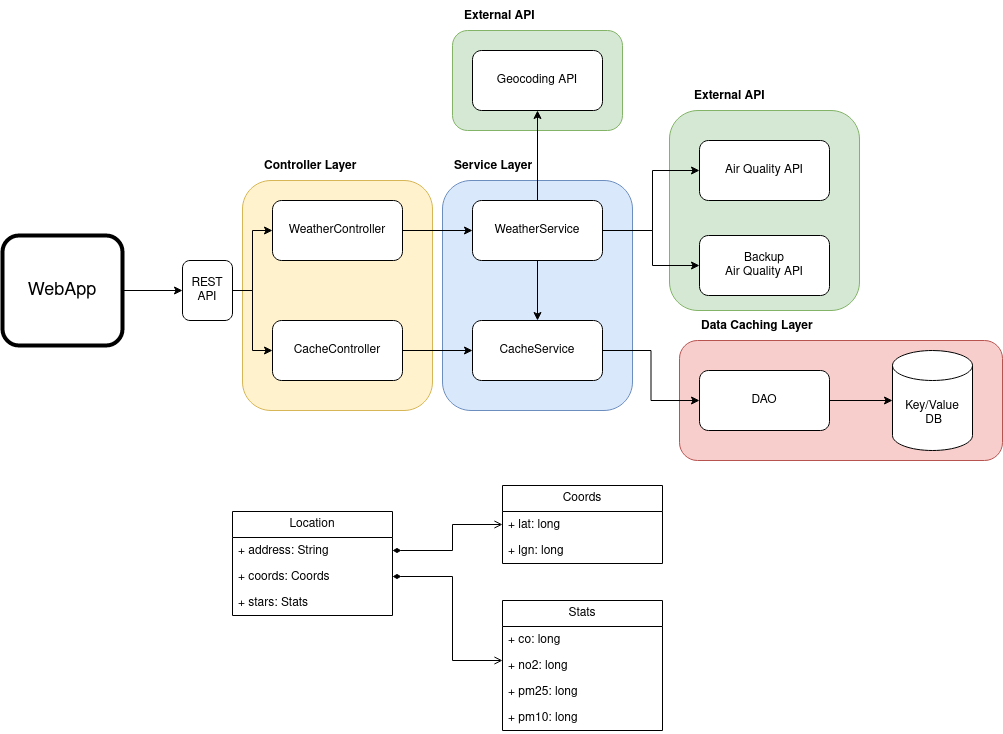
\includegraphics[scale=.4]{architecture.png}

\subsubsection{Technologies and API's Used}

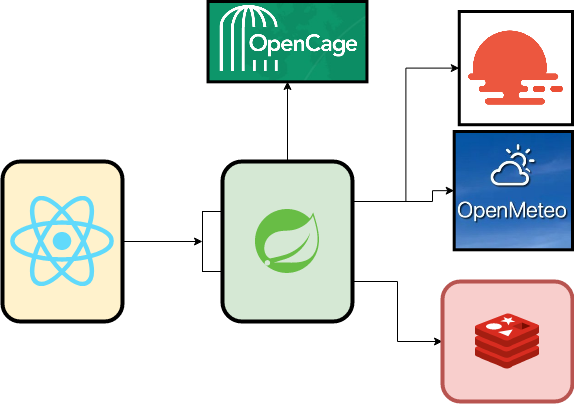
\includegraphics[scale=.4]{TechFrameworks.png}

\subsection{API for developers}

\section{Quality assurance}

\subsection{Logging}

Logging is a crucial aspect of software development that plays a vital role in supporting production and debugging activities. 

Logging was conducted using the slf4j Logger class has it provides an easy integration with the Spring Boot Application.

Each log message contains a timestamp, method invocation details, custom log messages, and other contextual data. Additionally, each log entry is assigned a logging level identifier, providing a way to categorize and prioritize log entries based on their significance.

I followed logging principles and best practices - such as: logging at the correct evel, providing meaningfull messages, etc - in order to provide meaningfull logs.

\subsection{Overall strategy for testing}

\subsection{Unit and integration testing}

\subsection{Functional testing}

\subsection{Code quality analysis}

SonarQube

\subsection{Continuous integration pipeline}

\section{References \& resources}

GitRepository can be found at \"my github\".

\subsection{Reference materials}

\end{document}